\documentclass{article}
\usepackage[normalem]{ulem}
\usepackage[utf8]{inputenc}
\usepackage{graphicx}
\usepackage{mathtools}
\usepackage{amssymb}
\usepackage{amsmath}
\usepackage{macros}
\usepackage{color}
\newcommand{\xa}{x-a}
\newcommand{\xan}[1]{(\xa)^{#1}}
\newcommand{\xab}{x^2+ax+b^2}
\newcommand{\xabn}[1]{(\xab)^{#1}}
\newcommand{\intx}[1]{\int^x_a{#1\ dt}}

\begin{document}

\section{Riemannintegralen}
Om man åker bil så har man en harstigetsmätare som mäter ens hastighet vid varje sekund.
Om man vill beräkna hur långt man har åkt, när hastigheten ej är konstant.

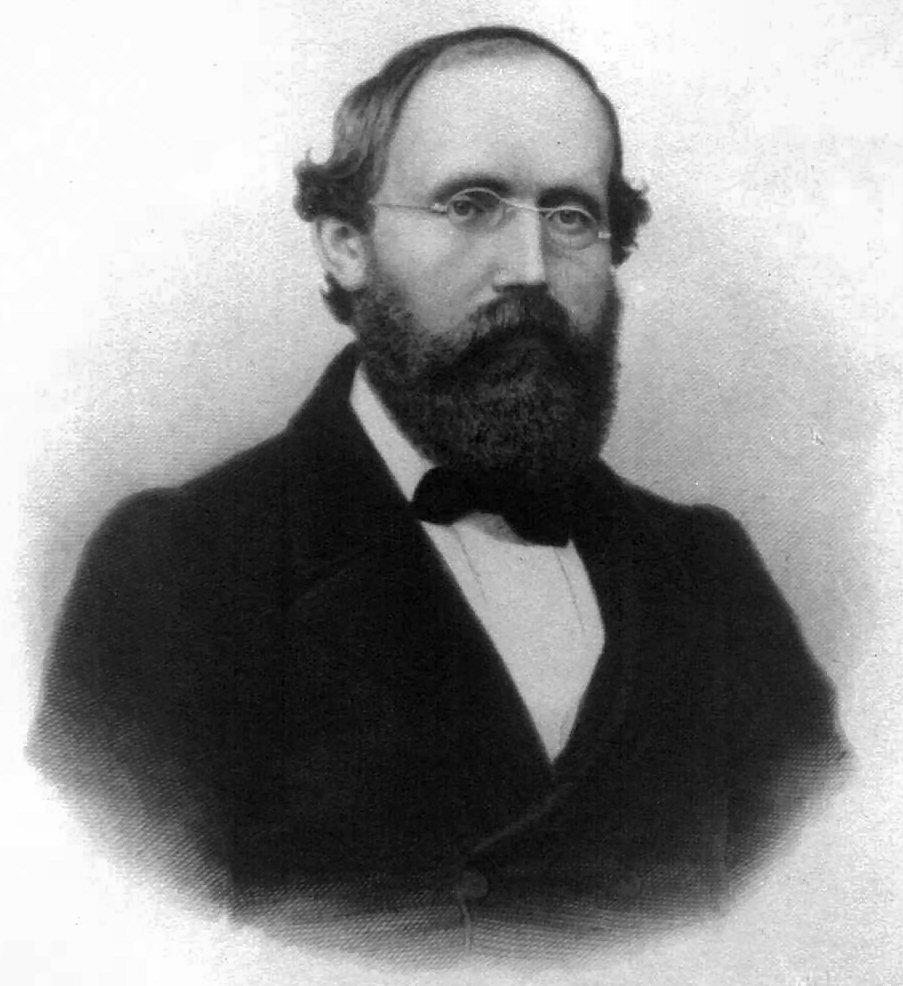
\includegraphics[scale=0.3]{img/riemann.jpeg}
\begin{verbatim}
Uppkom när man ville precicera definitionen av integraler
när fourier skapade fourier transformer
\end{verbatim}

\subsection{Definition}
En \uline{trappfunktion} på intervallet $[a, b]$ är en styckvis konstant funktion:\\
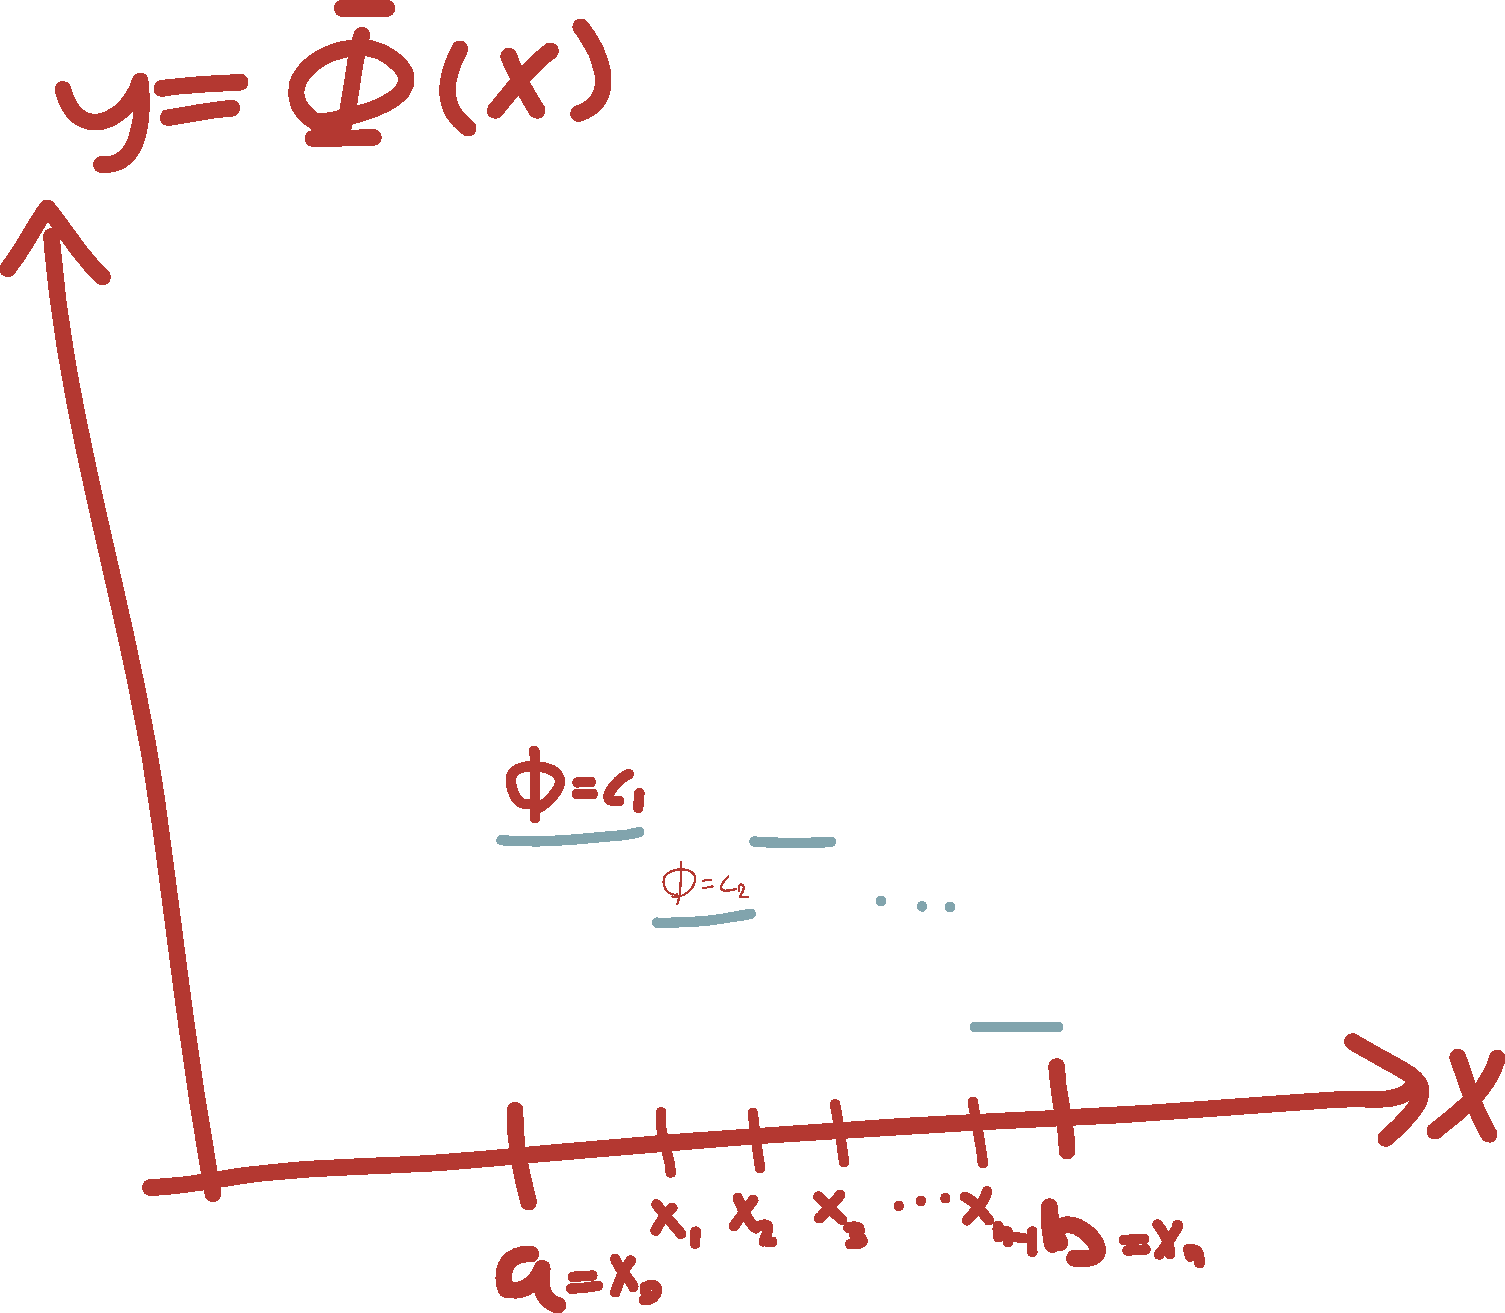
\includegraphics[scale=0.25]{img/img1.pdf}

Beteckna motsvarande \uline{trappsumma} med $T(\Phi)=\sum_{k=1}^n c_k (x_k-x_{k-1})$\\
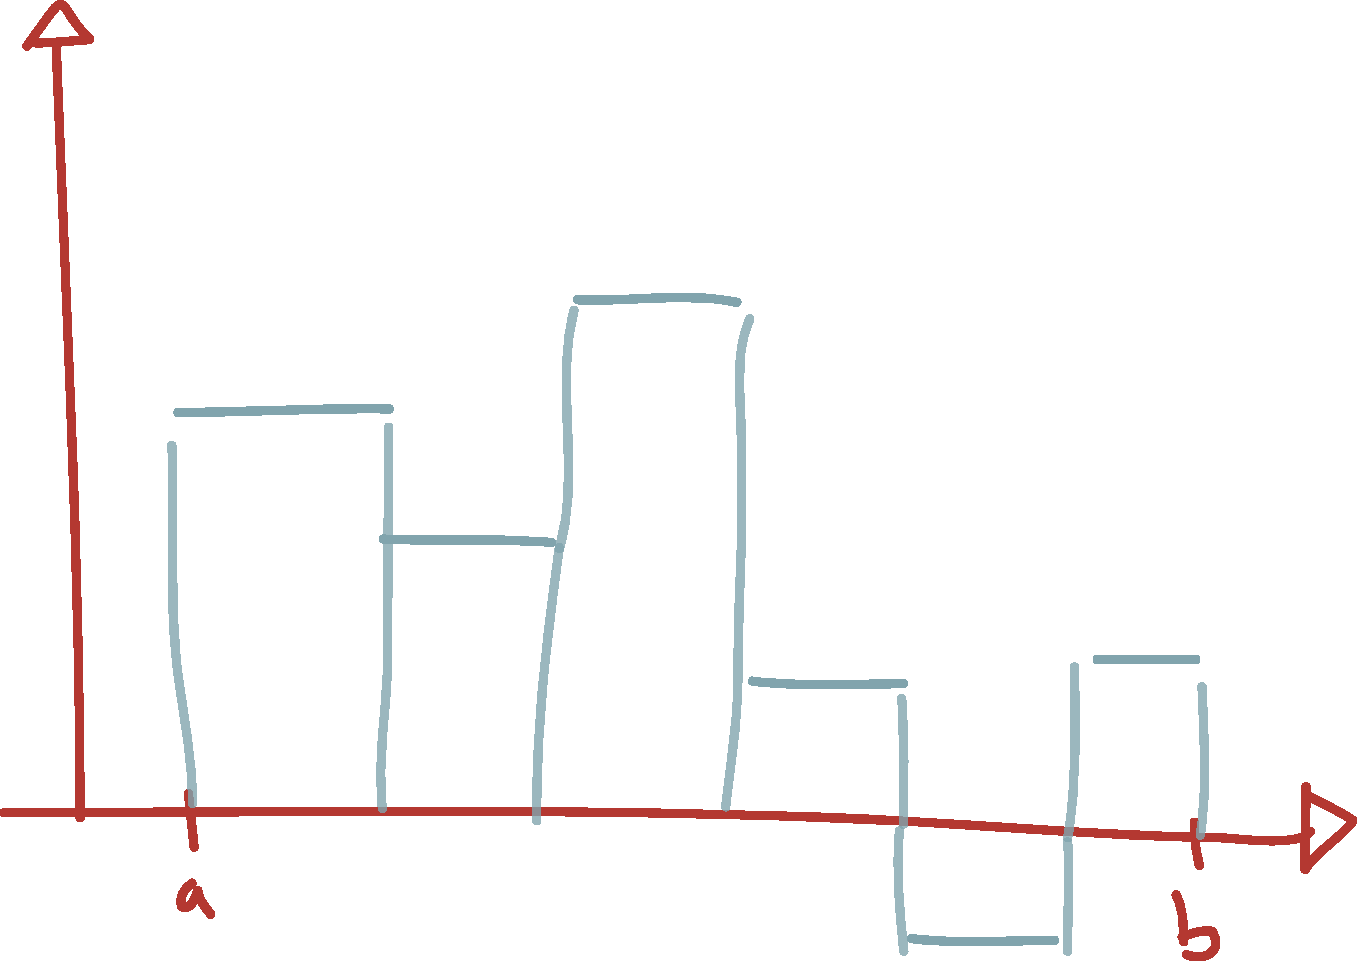
\includegraphics[scale=0.25]{img/img2.pdf}\\
Summa av rektangelareor ("med tecken").

\subsection{Definition}
En funktion $f$ sägs vara \uline{(Riemann)integrerbar} på intervallet $[a,b]$ om:

\begin{itemize}
  \item $f$ är deifinerad på $[a,b]$
  \item $f$ är begränsad på $[a,b]$ (dvs $\abs{f(x)}\le M$ för någon konstant M och alla $x\in [a,b]$)
  \item $f$ kan \uline{approximeras godtyckligt väl med trappfunktioner} i den meningen att det för varje $\epsilon>0$
    finns trappfunktionen $\Phi$ och $\Psi$ på $[a,b]$ sådana att $\Phi\le f \le\Psi$ och $T(\Psi)-T(\Phi) < \epsilon$.\\
    $\Phi$ = undertrappa (till $f$), $\Psi$ = övertrappa, $T(\Psi)$ = översumma, $T(\Phi)$ = översumma.
\end{itemize}
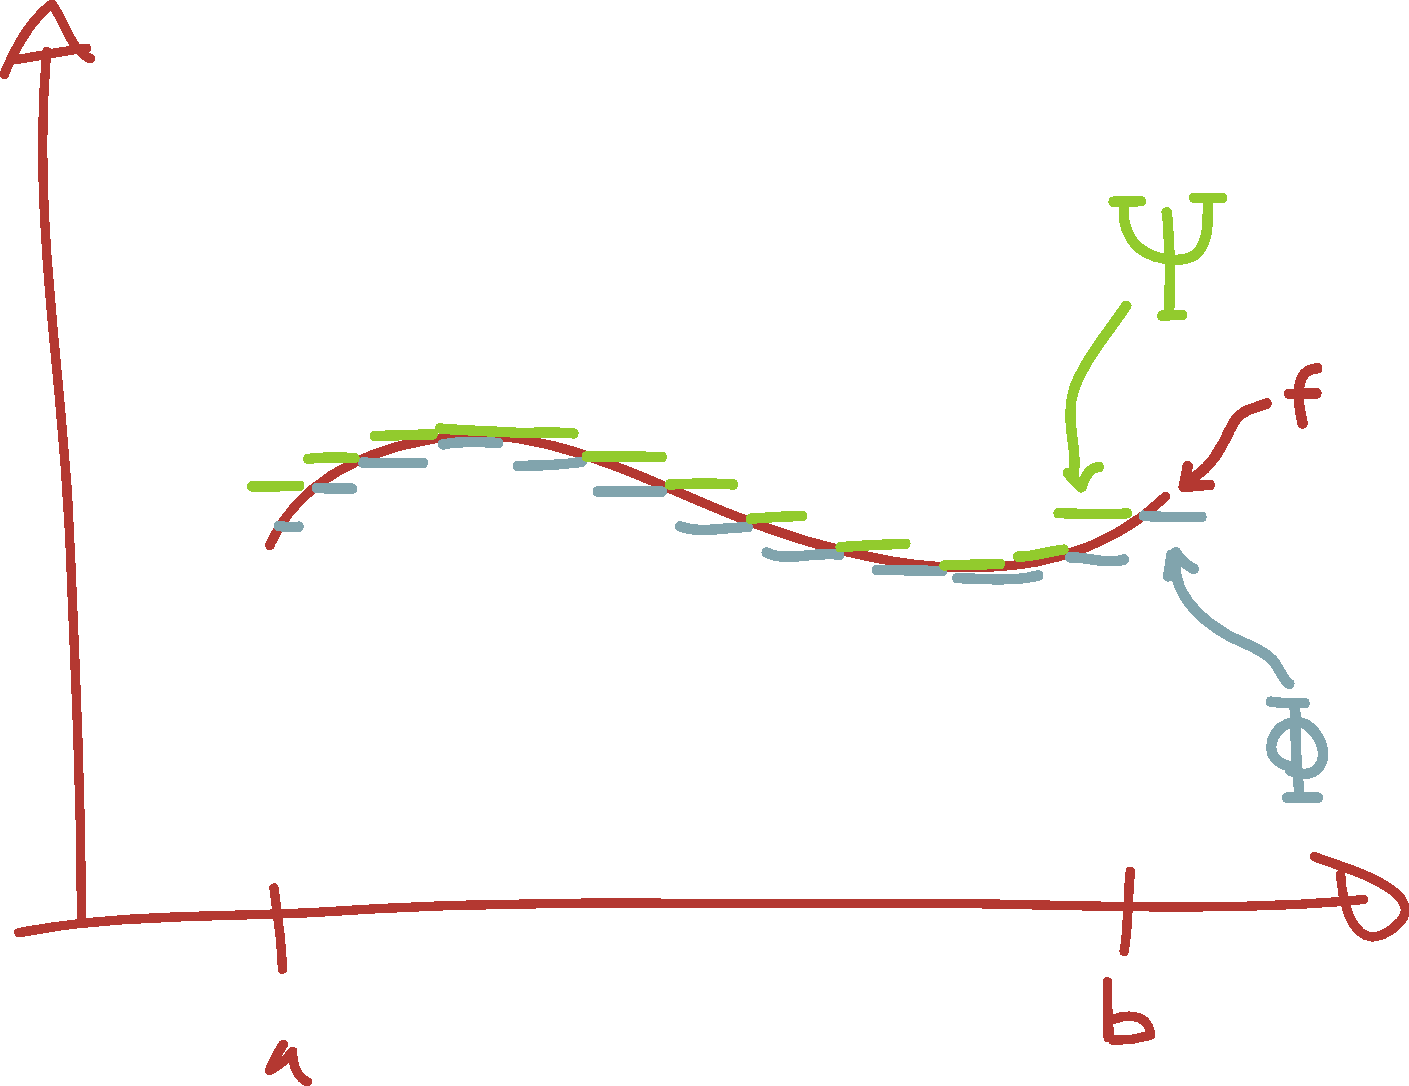
\includegraphics[scale=0.25]{img/img3.pdf}\\

I så fall är
$$\sup\{T(\Phi) : \Phi \le f\} = \inf \{T(\Psi) : f\le \Psi\}$$
och detta tal kallas för (Riemann)integralen för $f$ över intervallet $[a,b]$ och betecknas
$\int^b_a{f(x)\ dx}$ (eller $\int^b_a{f(t)\ dt}$ etc)

\subsection{Sats}
Styckvis kontinuerliga funktioner är integrerbara,
och även styckvis monotona funktioner.
(Bevis: Se boken)

Följande räknelagar bevis med hjälp av motsvarande egenskaper för trappsummor:

\subsection{Sats} Antag $f$ och $g$ integrerbara och $a<b<c$
\begin{itemize}
  \item Lineraitet $\int_a^b{\pa{k_1 f(x) + k_2 g(x)}dx} = k_1\int^b_a{f(x)\ dx} + k_2\int^b_a{g(x)\ dx}$
  \item Monotonicitet $f\le g$ på $[a,b] \im \Int{f(x)} \le \Int{g(x)}$
    \\(Notera speciellt integralen av en positiv funktion kan \uline{inte} bli negativ!)
  \item $\abs{\Int{f(x)}} \le \Int{\abs{f(x)}}$ (jfr triangelolikheten $\abs{a+b}\le \abs a + \abs b, \abs{\sum{a_k}}\le\sum{\abs{a_k}}$)
  \item $\int^c_a{f(x)} = \Int{f(x)} + \int^c_b{f(x) dx}$
\end{itemize}

\subsection{Anmärkning}
Den sista räknelagen gäller för alla a, b, c (oavsett ordning) ifall man deifinerar
$$ \int^a_a{f(x)\ dx}=0 $$ och $$\int^a_b{f(x)\ dx}\int^b_a{f(x)\ dx}$$

\subsection{Sats (Medelvärdessatsen för integraler)}
Om $f$ är kontinuerlig på $[a,b]$ så finns $\xi \in ]a,b[$ så att

$$ \Int{f(x)} = f(\xi)(b-a) $$

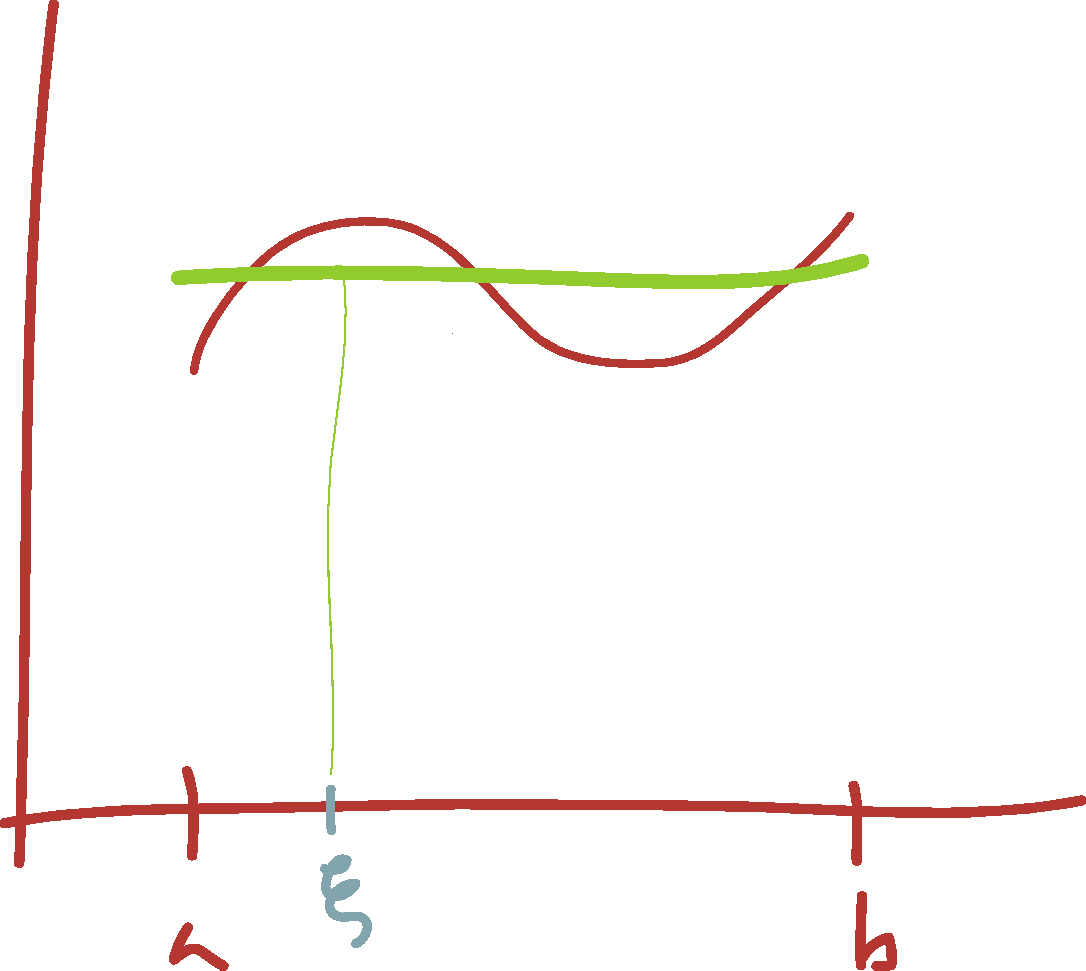
\includegraphics[scale=0.25]{img/img4.pdf}\\

($f(\xi)=$ medelvärdet för $f$ i $[a,b]$)
(Bevis: Se boken)

\subsection{Analysesns huvudsats}
Om $f$ är kontinuerlig så är $S(x) = \intx{f(t)}$ en primitiv funktion till $f$.

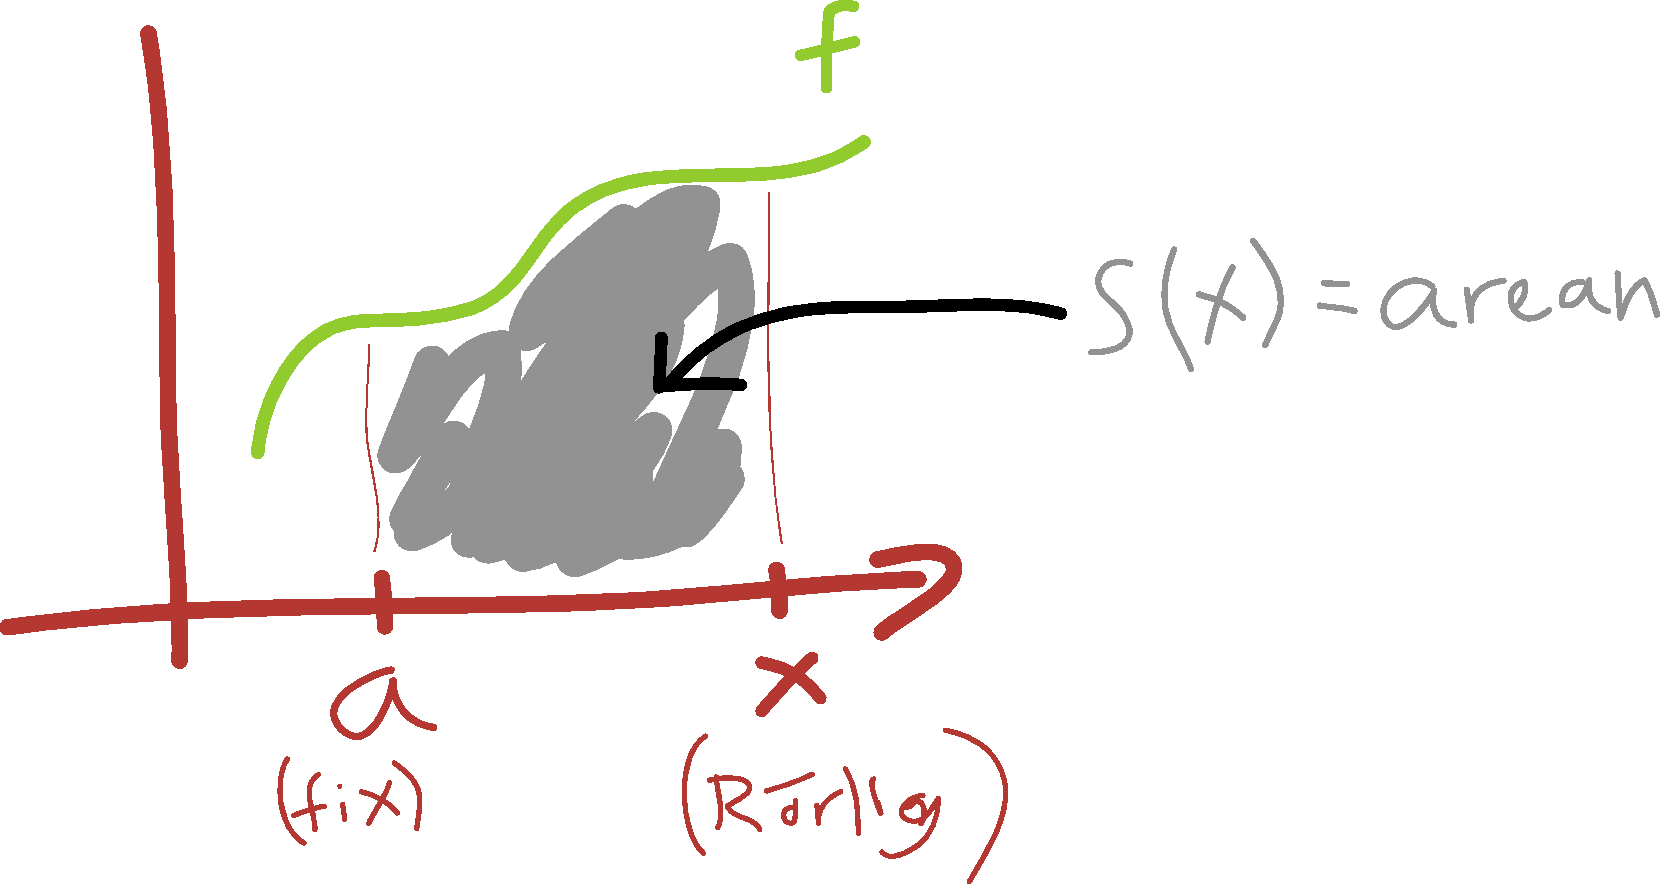
\includegraphics[scale=0.25]{img/img5.pdf}

\subsection{Bevis}
$$ \f{S(x+h) - S(x)}h = \f 1h \pa{\int_a^{x+h}{f(t)\ dt} - \intx{f(t)}} $$
$$ \f 1h\int^{x+h}_x{f(t)\ dt} = \f 1h f(\xi) h \to f(x), h \to 0$$

\subsection{Följdsats}
Varje kontinuerlig funktion har en primitiv funktion.

\subsection{Följdsats (insättningsformeln)}
Om $f$ är kontinuerlig och $F$ är en primitiv till $f$ så är $\Int{f(x)} = F(b)-F(a)$.\\
$ F(b)-F(a) $ skrivs ofta $\bra{F(x)}_a^b$.

\subsection{Bevis}
Sant enligt huvudsatsen ifall man tar $F(x)=S(x)=\intx{f(x)}$ som primitiv.
Tar man en annan primitiv $F(x)=S(x)+C$ så försvinner C i subtraktionen $F(b)-F(a)$,
så resultatet blir samma.

\subsection{Exempel}
Arean för $\int^2_1{x^2\ dx} = \bra{\f {x^3} 3}^2_1 = \f 83 - \f 13 = \f 73 $


\end{document}
